\section{Samostatná práce člena týmu\ --\ Vladimír Mečiar}
\label{sec:individual_work}

\subsection{Výběr tématu, popis provedeného průzkumu s uživatelem, analýza
uživatelských potřeb a klíčových problémů, navržená sada změn}

\subsubsection*{Výběr tématu}
\large{ Můj návrh:} \\
Plánovač, medicínský systém - lůžková část, rezervační systém \\
\noindent\large{ Vybraný návrh: }\\
Medicínský systém pro přihlašování klientů na procedury/sezení/vyšetření. Zaměření především na přihlašování klientů \\
a zobrazení těchto přihlášek

\subsubsection*{Analýza uživatelských potřeb a klíčových problémů}
\noindent\emph{Potřebné atributy rezervačního systému}
\begin{itemize}
    \item Přehled služeb a cen jednotlivých služeb
    \item Přehled zaměstnanců
    \item Přehled pracovní doby
    \item Přehled obsazenosti a volných termínů
    \item Vytváření a rušení termínů
    \item Přehled informací o rezervovaném termínu - jaká služba byla zvolená, jaký zaměstnanec a čas, jméno a kontaktní údaje zákazníka
    \item Ukazovatel času dne - Zvlášť vyobrazení uplynulých a nadcházejících termínů
    \item Informování o vytvoření rezervace - pro zákazníka i pro poskytovatele (cena, zaměstnanec, čas)
\end{itemize}
\newpage

\subsubsection*{Analýza existujících řešení}
\noindent\emph{Parkhotel - Pero, papír, telefon a recepční:}
\begin{itemize}
    \item[+] Jednoduché pro zákazníka
    \item[+] Komunikace s člověkem - zákazník se může zeptat na další případné informace
    \item[+] Recepční se může zeptat na další dodatečné informace (preference termínů, zaměstnanců atd)
    \item[-] Náročné udržování databáze - kniha
    \item[-] Vytvoření rezervace je pro poskytovatele náročné, zdlouhavé => nákladné
    \item[-] Přesun a rušení rezervace - náročné, zdlouhavé => nákladné
    \item[-] Nutnost osoby/osob zodpovědných za rezervace - člověk je tvor omylný
    \item[-] Možnost vytvoření rezervace jen v čase, kdy zaměstnanec pracuje
\end{itemize}

\noindent\emph{Holičství - Rezervační systém (visblee.sk)}
\begin{itemize}
    \item[+] Intuitivní a jednoduchý postup
    \item[+] Jasný přehled informací (ceny, služby, popis ... )
    \item[+] Posílání informací o vytvoření rezervace  - zaměstnancem i klientem
    \item[-] zvlášť webová aplikace - problematické přepojení s vlastní stránkou
    \item[-] problém s dostupností stránky (jak se tam dostat ?)
    \item[-] cena - podle počtu zaměstnanců, existují levnější řešení
    \item[-] pole poznámka - když má zákazník nějaké specifikace, často na ně zapomene nebo je neumí popsat
\end{itemize}

\noindent\emph{Holičství - Rezervační systém (rezerver.cz)}
\begin{itemize}
    \item[+] Intuitivní a jednoduchý postup
    \item[+] Jasný přehled informací (ceny, služby, popis ... )
    \item[+] Zasílání informací o vytvoření rezervací  - zaměstnancům i klientům
    \item[-] Vytvořená stránka na zakázku - nedá se použít pro vícero poskytovatelů služeb
\end{itemize}

\subsection{Popis provedeného průzkumu s uživatelem}
Průzkum byl provedený s uživateli rezervačních systémů: \\
wellness v Parkhotelu na Baračke a holičství v Brně.
V případě hotelu se jednalo jen o pero a papír, zatímco holičství používalo webovu aplikaci. S~uživateli byl vedený rozhovor.
Uživatele jsem požádal o demonstraci vytvoření rezervace a její následné zrušení. Na konci jsem se uživatele zeptal na jeho postřehy a názory.\\

\subsection{Popis současného řešení - jaké nástroje uživatel používá, \\
popř. obrázky/screenshoty současného řešení/reálné situace}

\noindent\emph{Parkhotel - rezervace klienta}
\begin{itemize}
    \item Klient zavolal na recepci hotelu s žádostí o wellness službu (viz \ref{fig:parkhotel_wellnes_services})
    \item Recepční na hotelu se telefonicky spojil s wellness a zeptal se na dostupnost služby(viz \ref{fig:parkhotel_wellnes_database})
    \item Recepční zavolal zpět klientovi a oznámil mu dostupnost služby, případně i službu objednal
    \item V případě zrušení nebo jakýchkoliv jiných změněných okolností dalo wellness vědět recepčnímu a ten dal následně vědět klientovi
\end{itemize}

\noindent\emph{Holičství - rezervace klienta}
\begin{itemize}
    \item Klient se "proklikal" webovou aplikací a objednal se sám (viz \ref{fig:barber})
    \item Klient zavolal do holičství a recepční ho objednal na termín
    \item Klientovi přišel e-mail s informacemi o vytvoření rezervace
    \item Recepčnímu se zobrazovaly jednotlivé termíny rezervací v tabulce a mohl je upravovat (t.j rušit, přidávat nové)
    \item V případě zrušení termínu byl zákazník informovaný a to podle potřeby e-mailem nebo telefonicky
\end{itemize}
\newpage


\begin{figure}[h]
    \begin{subfigure}{.5\textwidth}
        \centering
        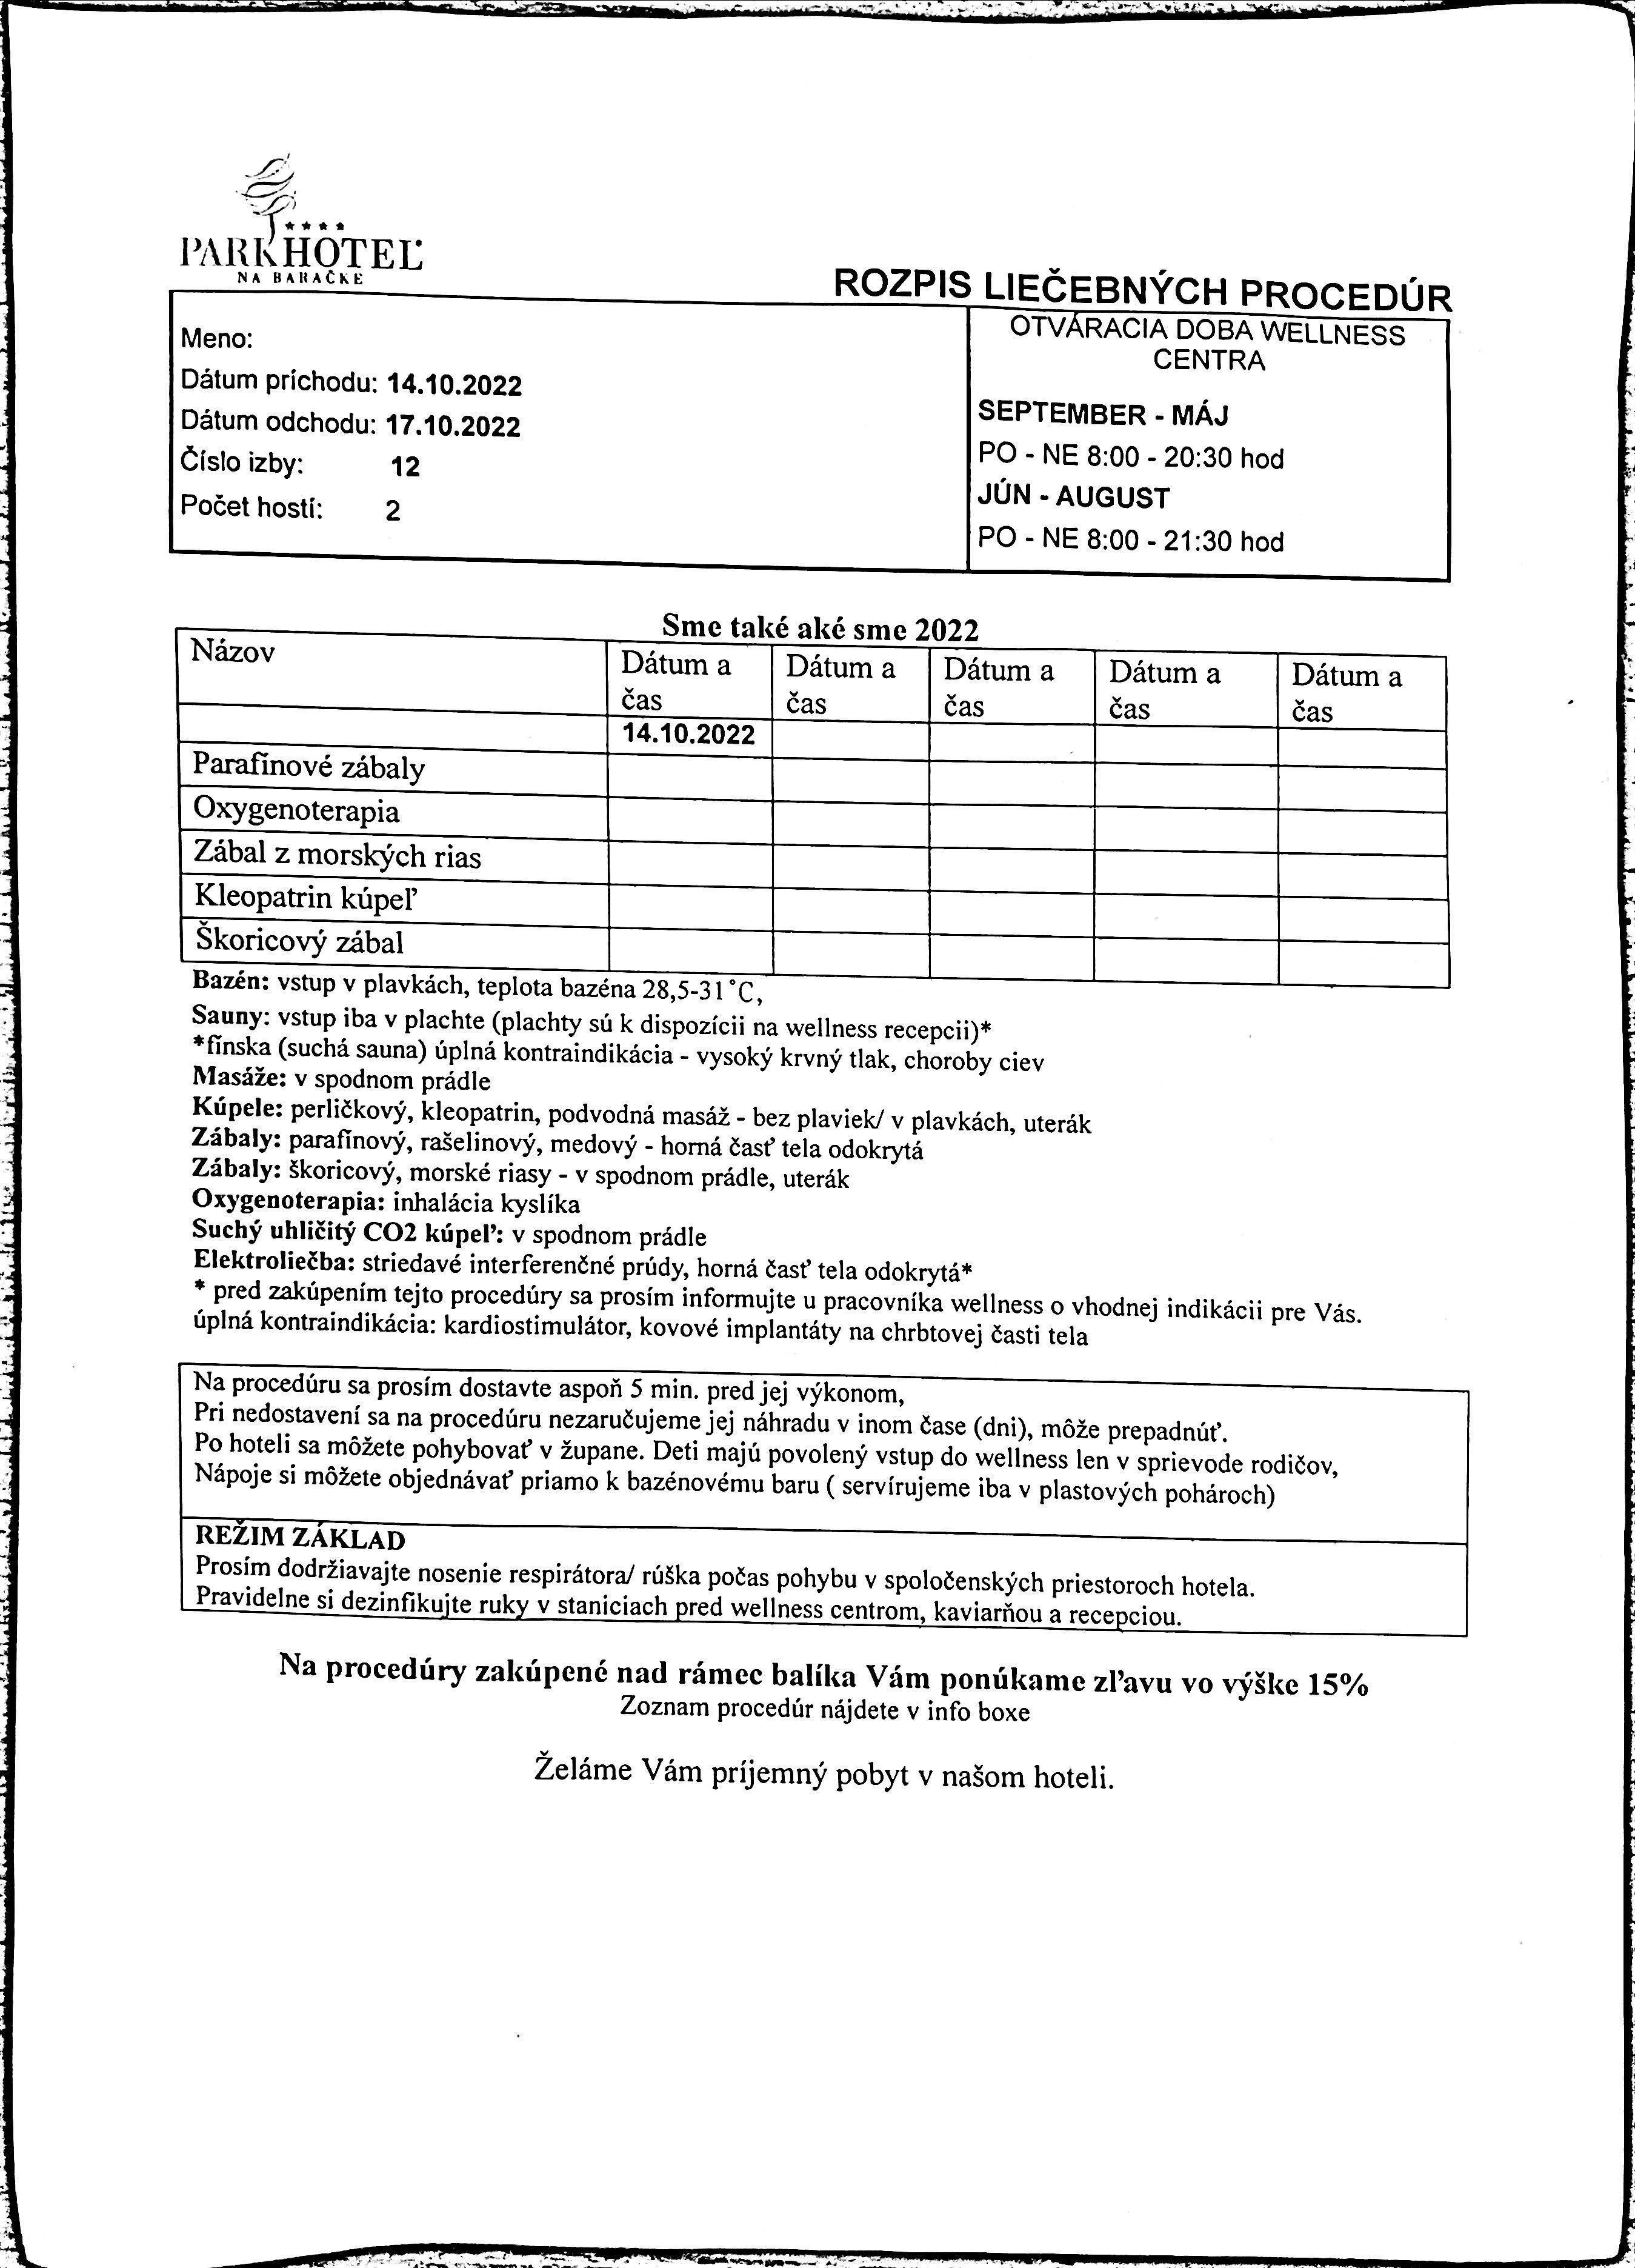
\includegraphics[width=.4\linewidth]{doc/latex/fig/vlado/IMG_9344.jpg}
        \caption{Nabídka služeb}
        \label{fig:parkhotel_wellnes_services}
    \end{subfigure}
    \begin{subfigure}{.5\textwidth}
        \centering
        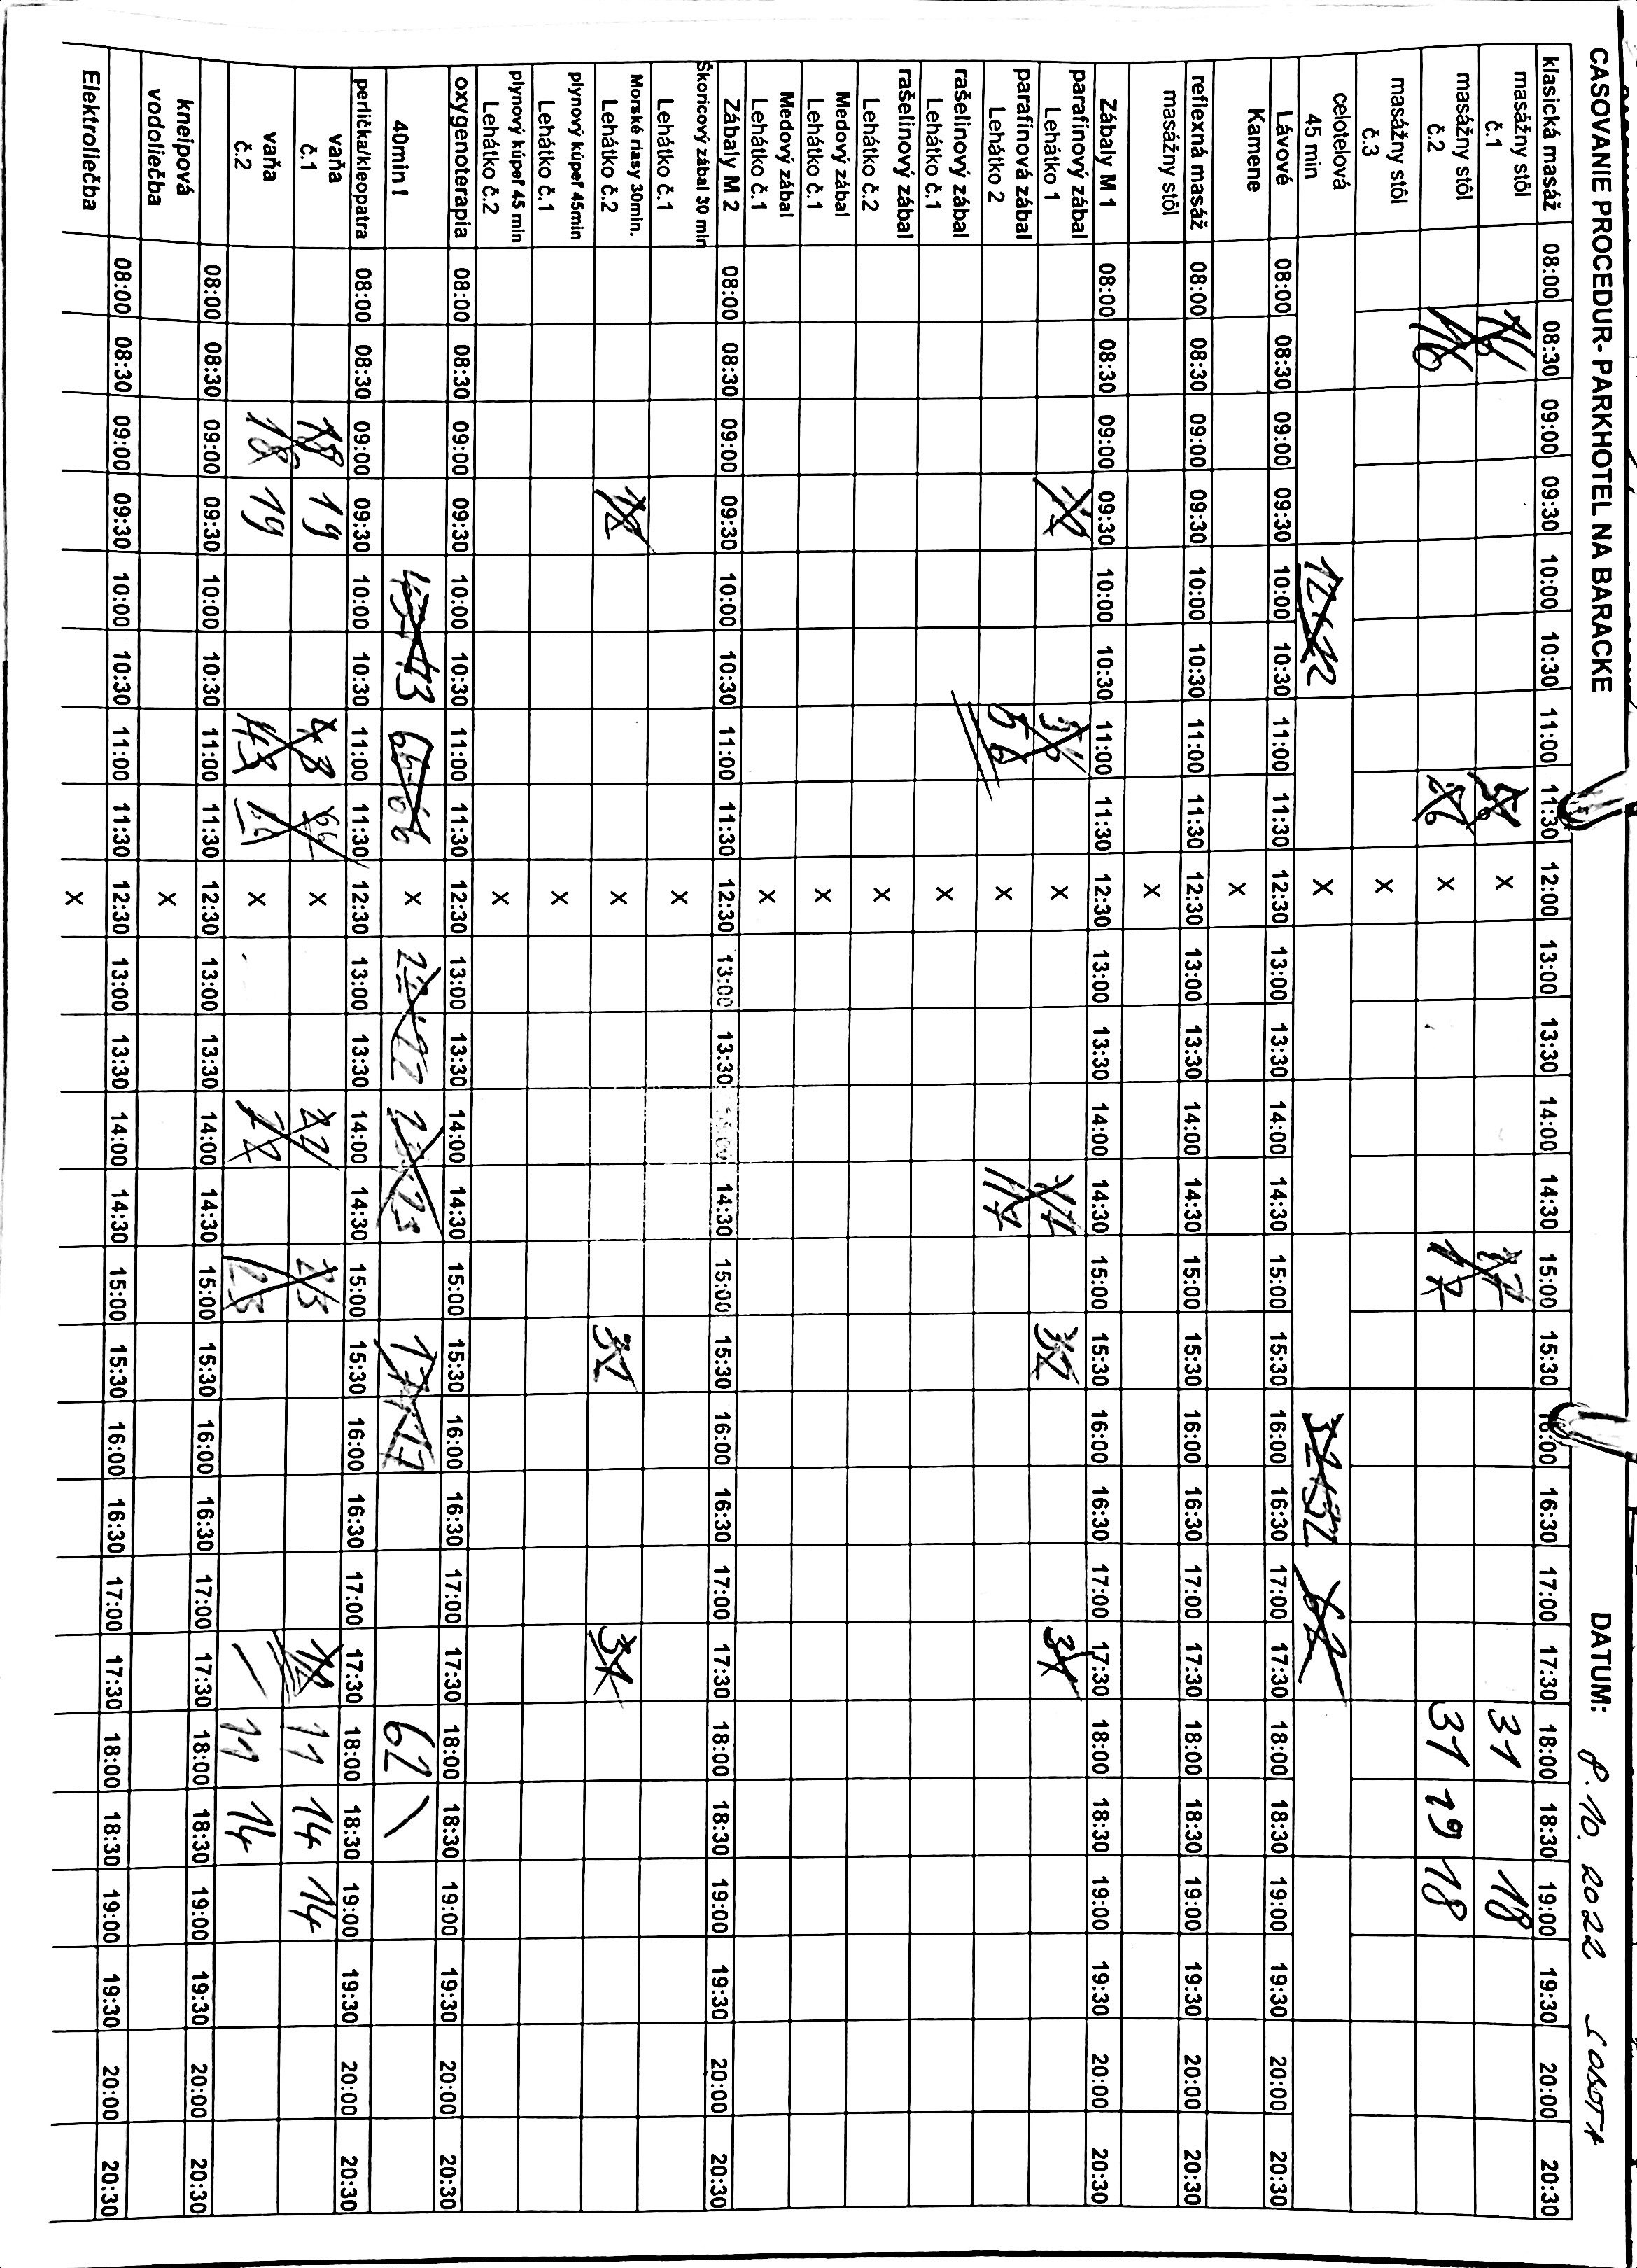
\includegraphics[width=.4\linewidth]{doc/latex/fig/vlado/IMG_9343.jpg}
        \caption{Databáze wellness}
        \label{fig:parkhotel_wellnes_database}
    \end{subfigure}
    \caption{Parkhotel}
    \label{fig:parkhotel}
\end{figure}

\begin{figure}[h]
    \begin{subfigure}{.5\textwidth}
        \centering
        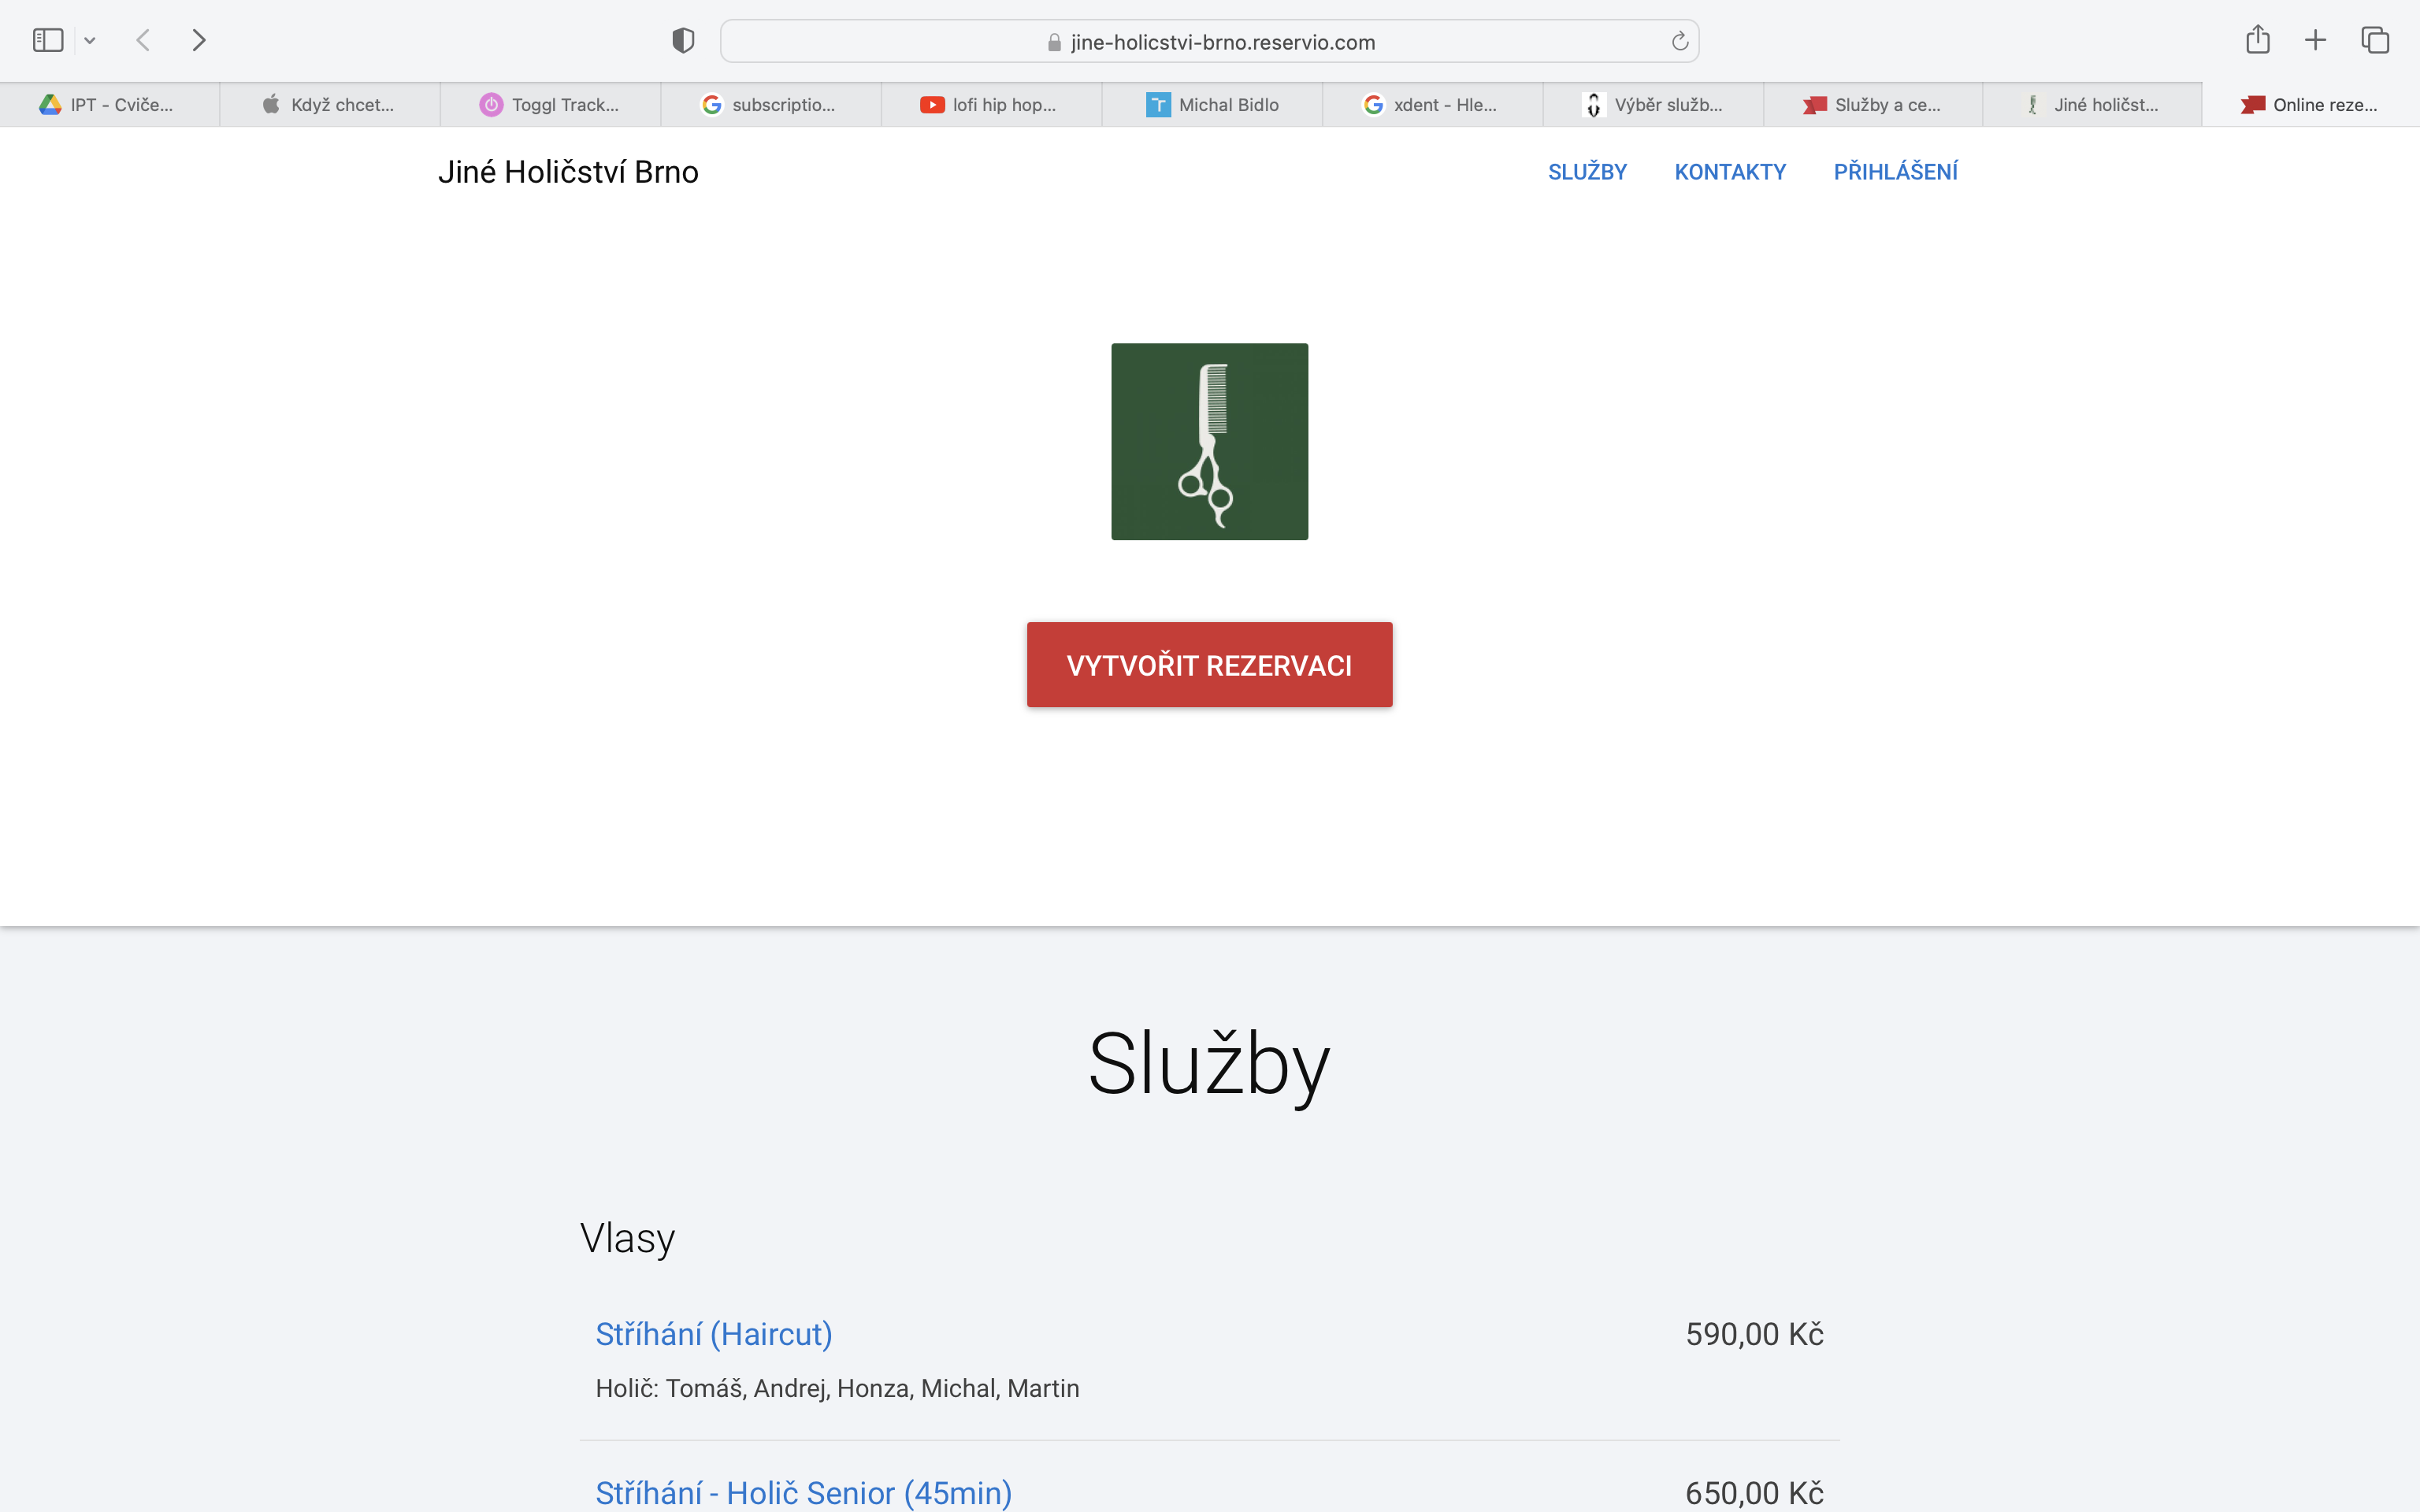
\includegraphics[width=.8\linewidth]{doc/latex/fig/vlado/rezervio_cz.png}
        \caption{Aktuálně používaná webová aplikace}
        \label{fig:current_aplication}
    \end{subfigure}
    \begin{subfigure}{.5\textwidth}
        \centering
        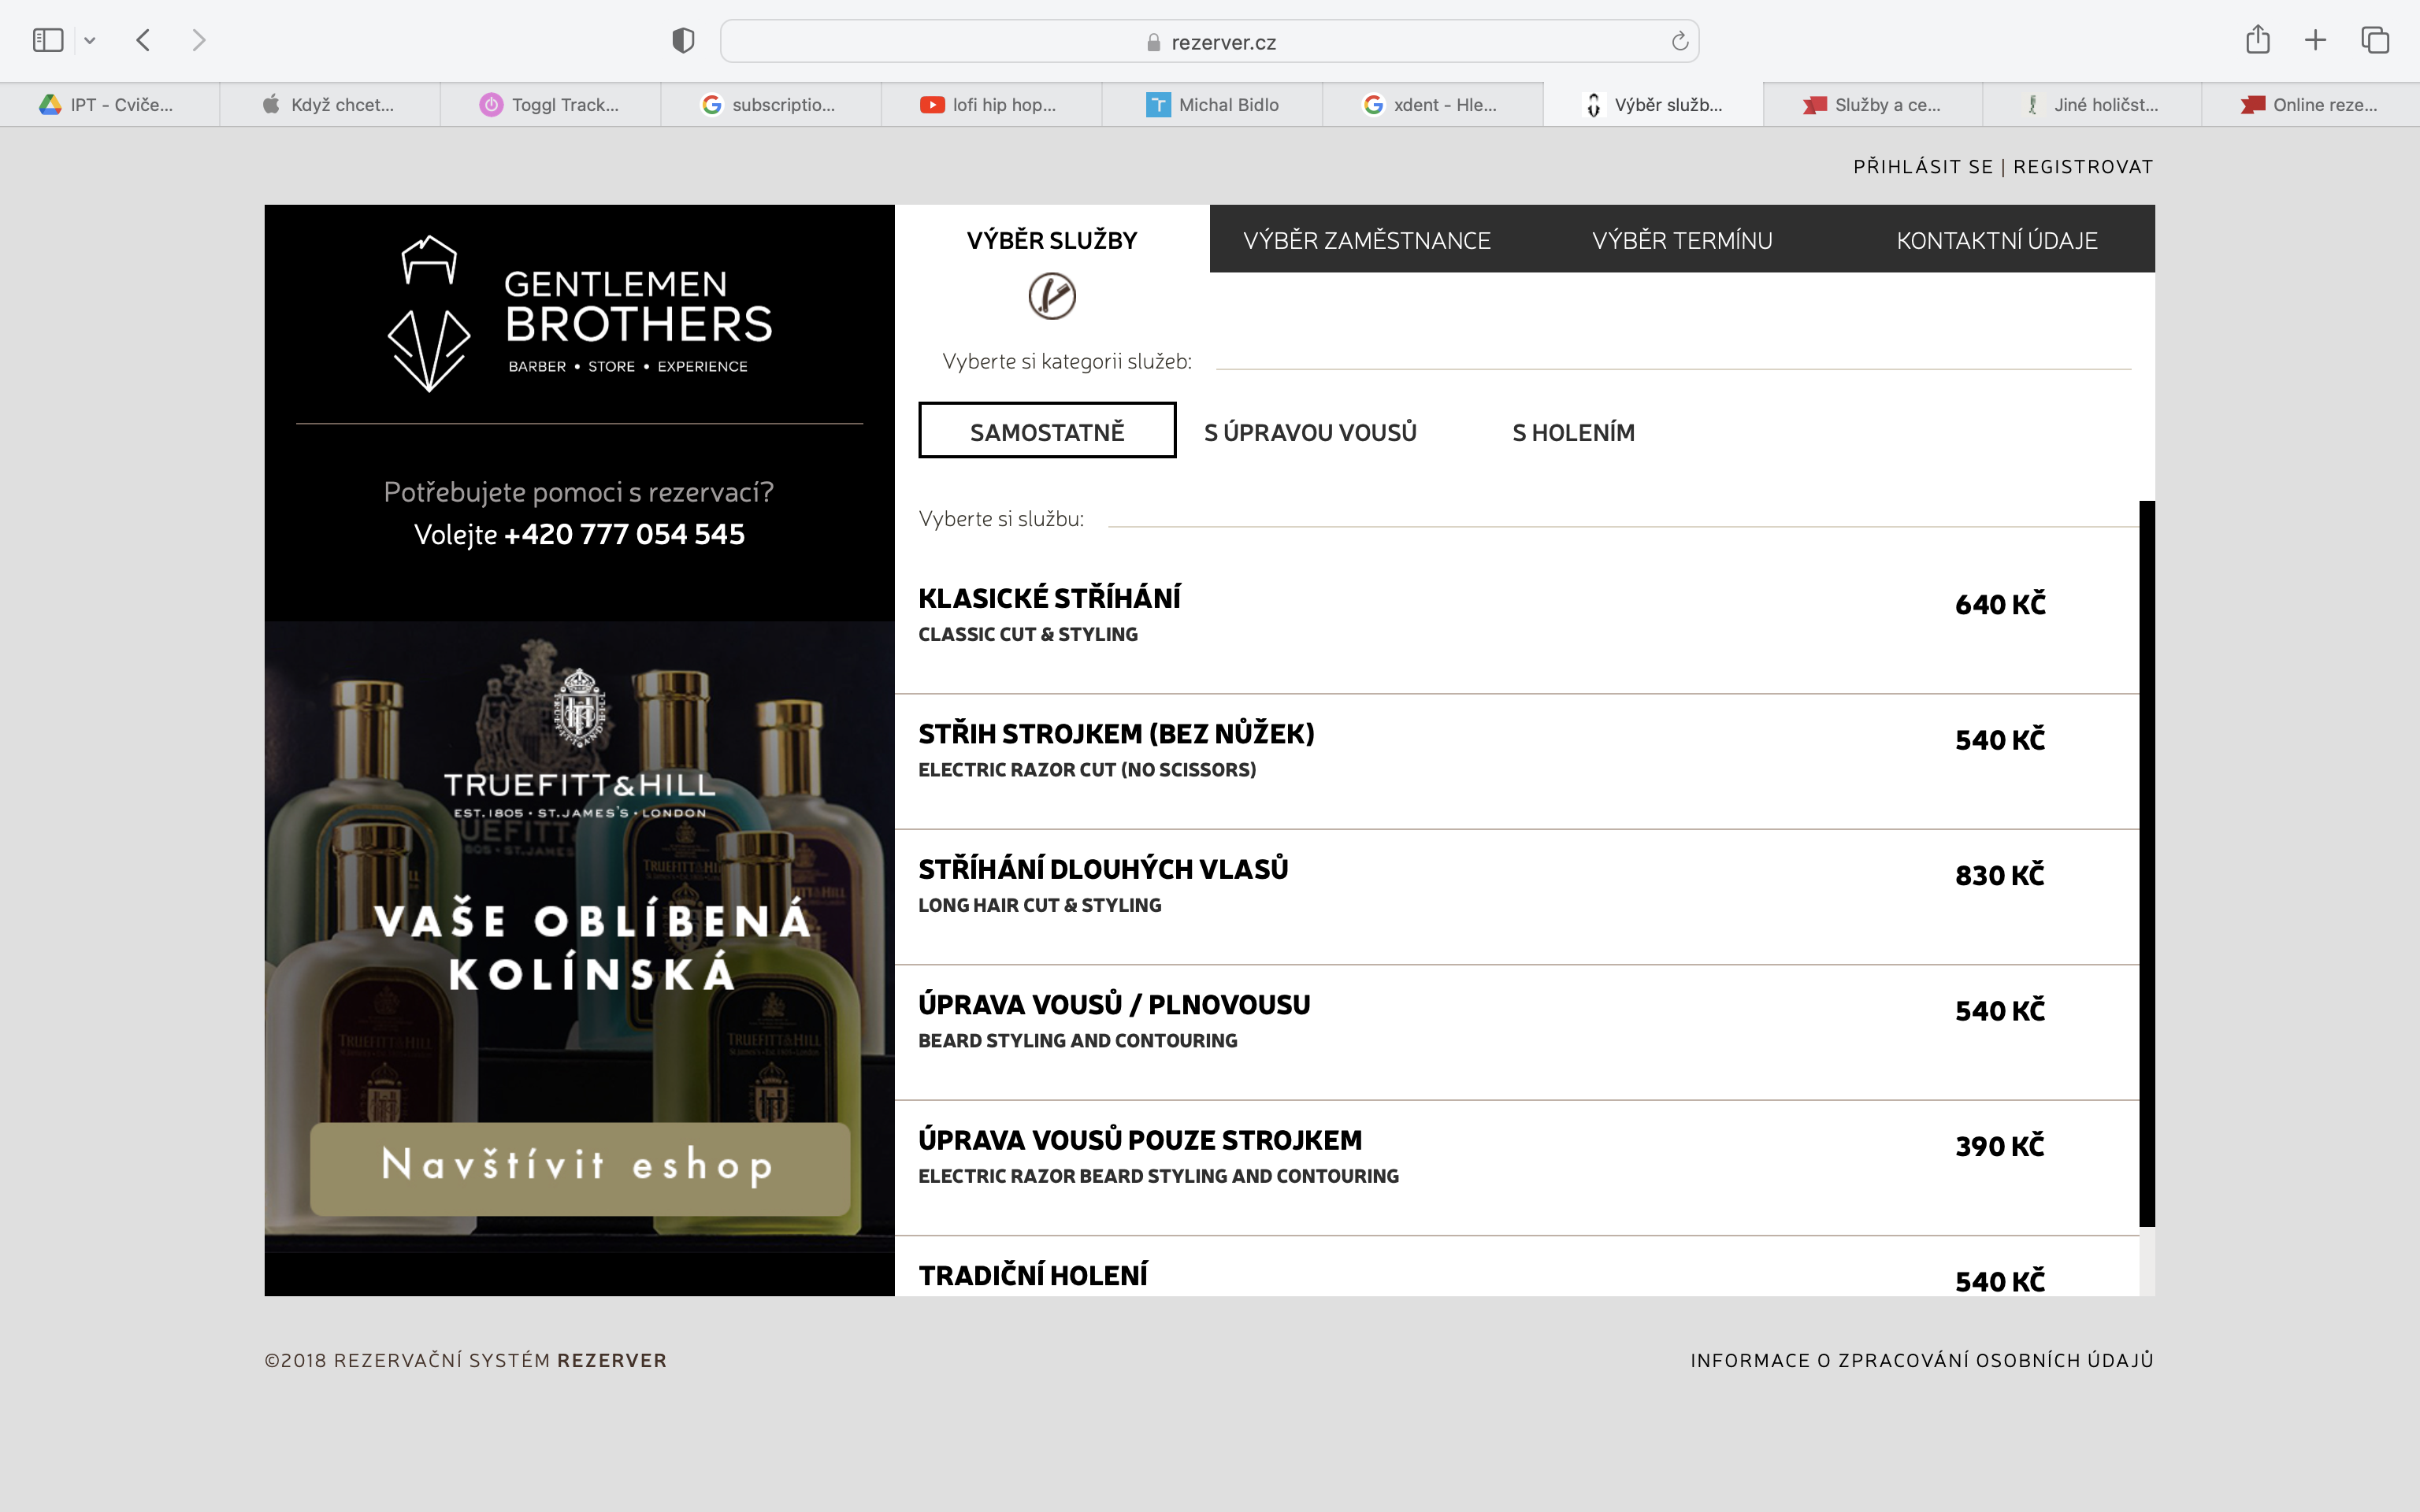
\includegraphics[width=.8\linewidth]{doc/latex/fig/vlado/rezerver_cz.png}
        \caption{Předchozí webová aplikace}
        \label{fig:previous_aplication}
    \end{subfigure}
    \caption{Holičství}
    \label{fig:barber}
    \centering
    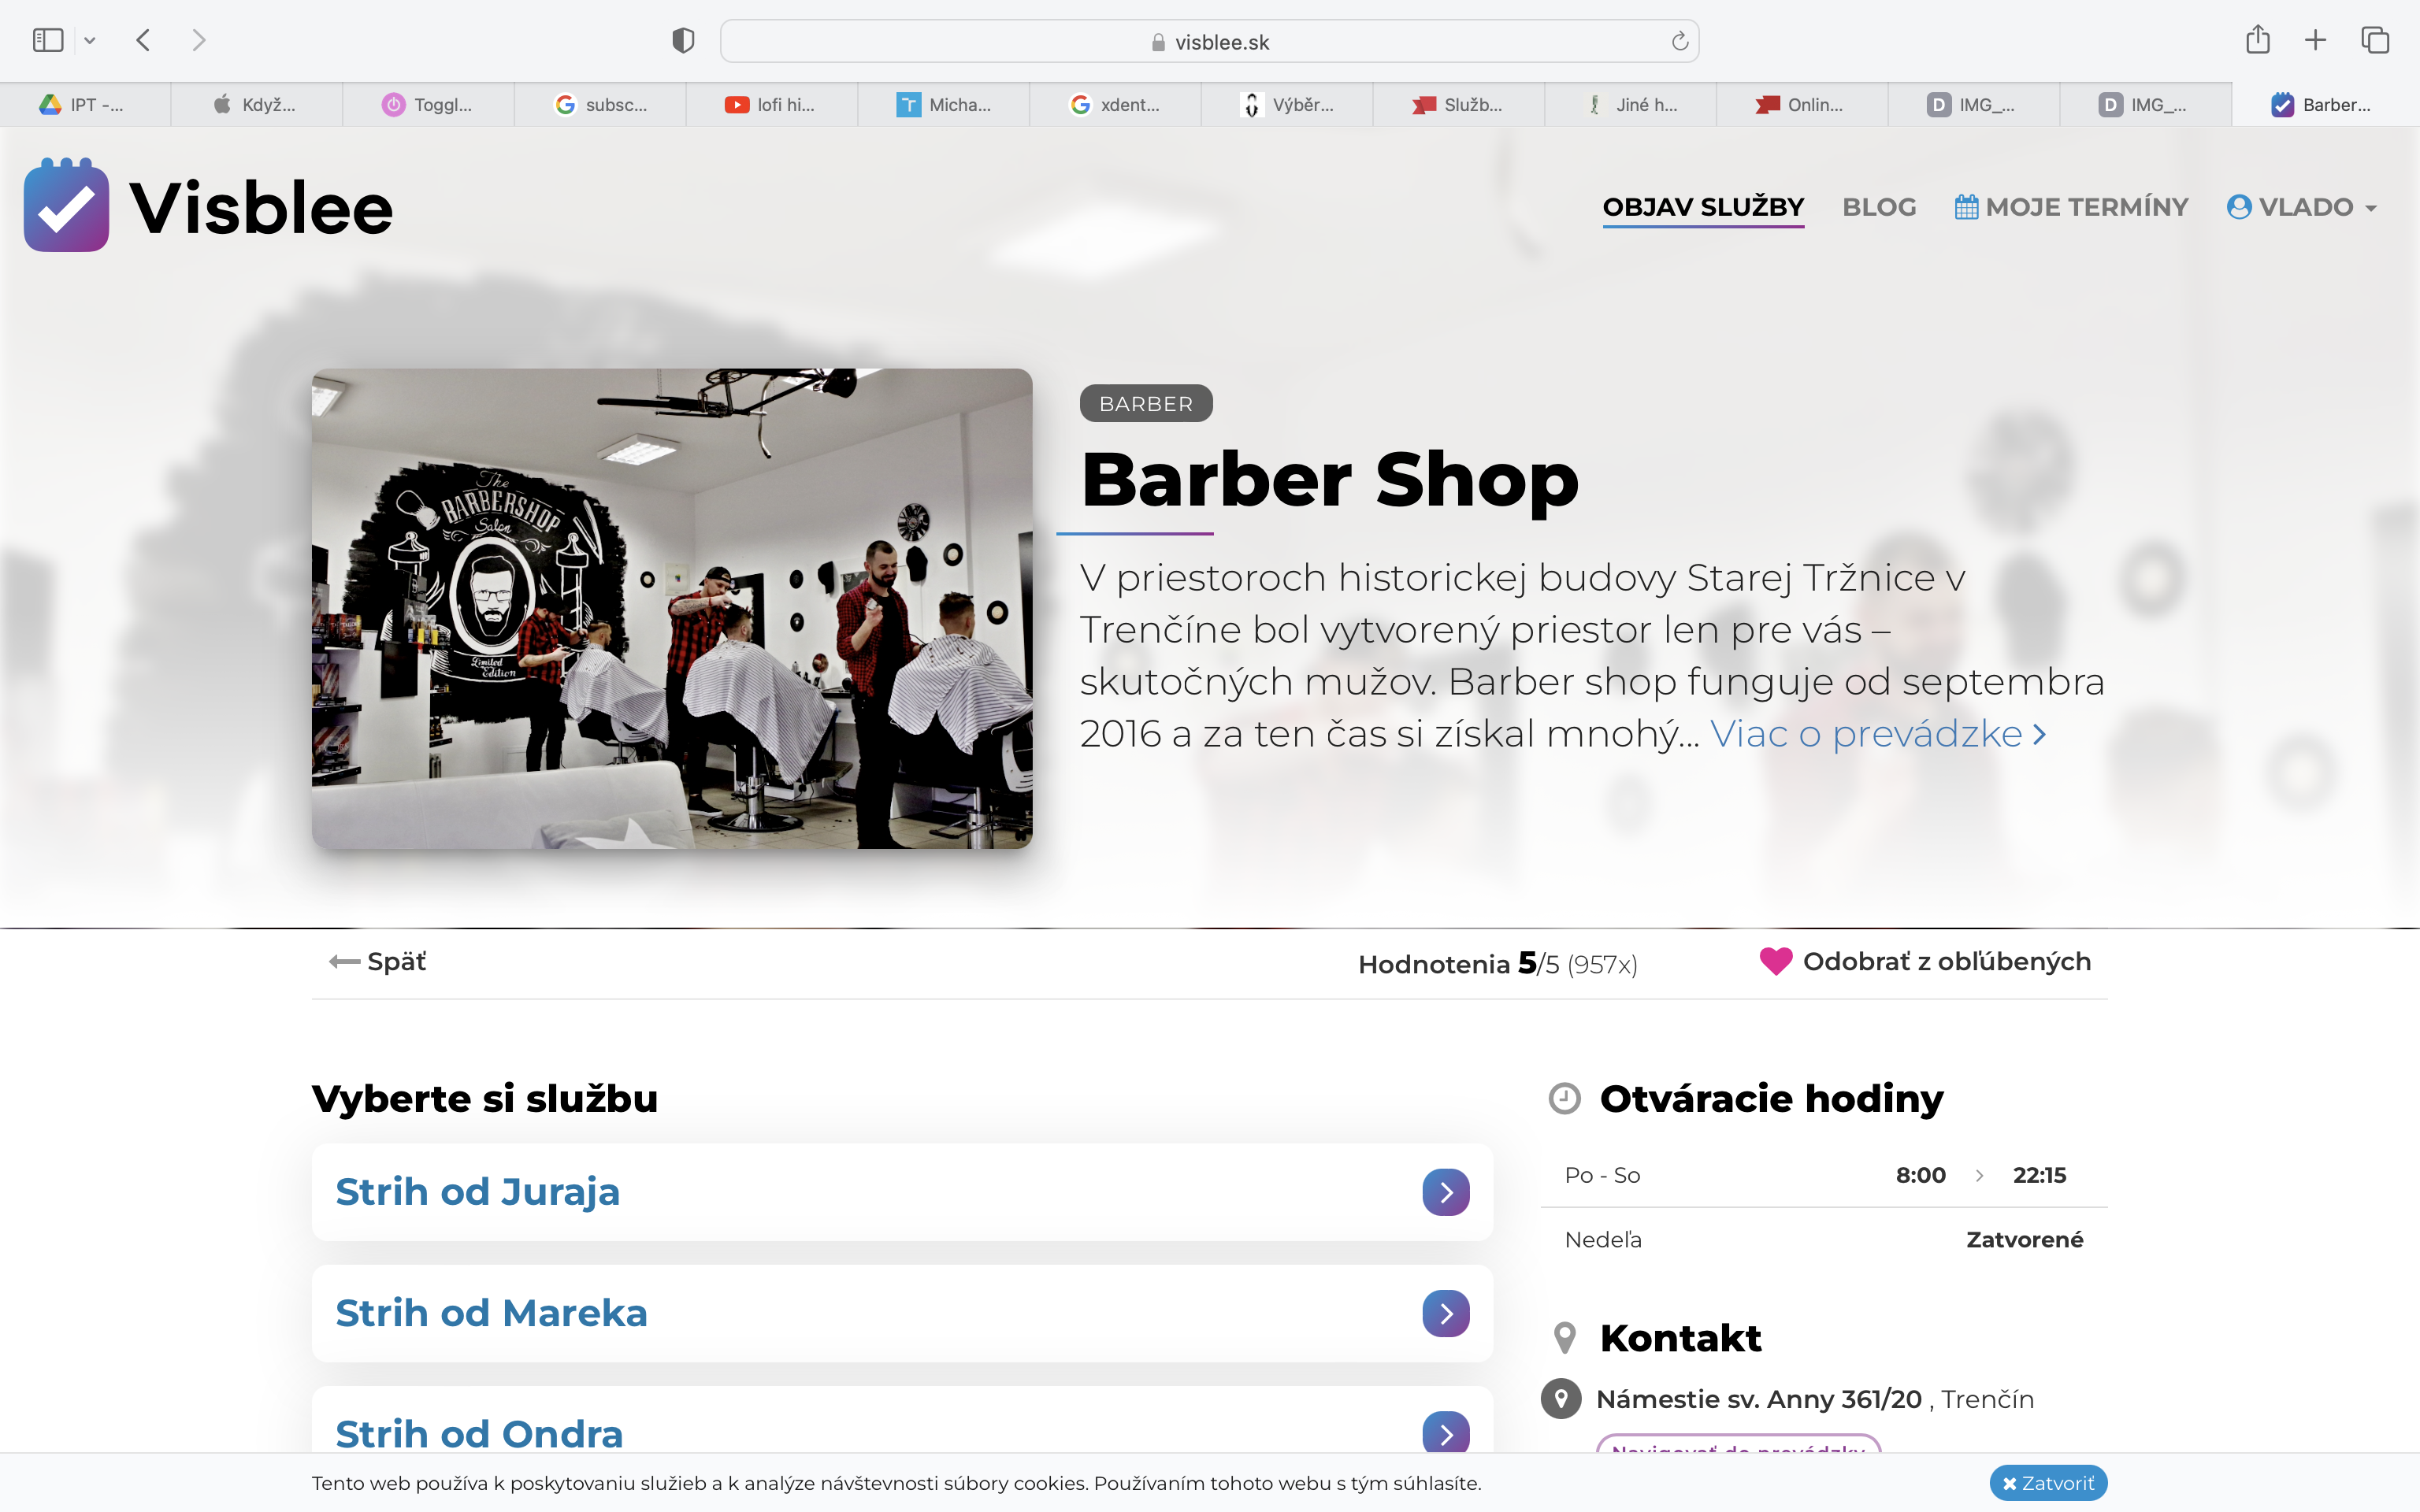
\includegraphics[width=.4\linewidth]{doc/latex/fig/vlado/visblee_sk.png}
    \caption{Aplikace visblee}
    \label{fig:visblee}
\end{figure}
\newpage

\subsubsection*{Navržená sada změn}
Každá z vybraných aplikací a postupů má svoje výhody

\noindent\emph{Jedna aplikace:}
\begin{itemize}
    \item ponechat jednoduchost - dobře zvolit konkrétní postupy rezervací\\ internetových aplikací ponechat v naší
    \item základní funkcionalita - aby bylo možné vytvářet rezervace - potom případně rozšiřovat o další funkcionalitu (statistiky apod.)
    \item vytvořit stylem "plugin" - jedno řešení schopné přepojit se už s internetovou stránkou (možná i v rámci databáze)
    \item Kompatibilita - co nejvíce prohlížečů a zařízení => vytvoření jednoho univerzálního rozšíření pro poskytovatele služeb
\end{itemize}

\subsection{Návrh uživatelského rozhraní, makety rozhraní, testování pomocí maket rozhraní}

\subsubsection{Návrh uživatelského rozhraní}
\noindent\emph{Část projektu v týmu: Návrh rozhraní pro klienty}\\
Rozhraní nově vytvářené aplikace bylo inspirované aplikací resrvio.cz (\ref{fig:current_aplication}). Na~základě průzkumu
mezi uživateli internetové aplikace (konkrétně klienty) jsme se rozhodli použít identický postup rezervace.

\subsubsection{Makety rozhraní}
Maketa rozhraní ponechá jednoduchost a intuitivnost aplikace reservio.cz \ref{fig:current_aplication}. Prvotní prvek (tlačítko)
bude "připojený" k internetové stránce. Zákazník se přes něj bude moct dostat přes jednotlivé kroky rezervace.  \\
To konkrétně:\\
\begin{itemize}
    \item[1] Výběr služby, nejprve pomocí primární služby a potom výběr jednotlivých podsekcí služby
    \item[2] Výběr zaměstnance
    \item[3] Výběr data a času
    \item[4] Doplnění údajů (neplatí pro přihlášeného uživatele)
    \item[5] Potvrzení o vytvoření rezervací modulárním oknem a přesměrování na původní stránky poskytovatele služeb
\end{itemize}


\newpage
\begin{figure}[h]
    \centering
    \includegraphics[width=1.4\textwidth, angle=270]{doc/latex/fig/vlado/Reservation_client_part-1.pdf}
    \caption{Navržená maketa}
    \label{fig:mokcup}
\end{figure}
\newpage

\subsubsection{Testování pomocí maket rozhraní}
Testování rozhraní proběhlo v aplikaci Figma na spolužácích v týmu a mých známých kteří mi
pomohli napravit nedostatky. Věřím, že s jejich pomocí byla vytvořená co nejlepší maketa.

\newpage
